\section{Laboratory work implementation}

\subsection{Tasks and Points}

- Realizeaza un simplu GUI calculator care suporta urmatoare functii: +, -, /, *, putere, radical, InversareSemn(+/-), operatii cu numere zecimale.\\
\indent 
- Divizare proiectului in doua module - Interfata grafica(Modul GUI) si Modulul de baza(Core Module).

\subsection{Analiza lucrarii de laborator}
\selectlanguage{russian}
В ходе данной лабораторной работы был разработан калькулятор. При разработке использовалось IDE Microsoft Visual Studio 2013. Программа написана на языке C\#.\\
\indent 
Разработка производилась в 2 этапа:\\
\indent 
1) Внешний интерфейс;\\
\indent 
2) Функционал.\\
\indent 
Microsoft Visual Studio обладает всем необходимым функционалом для удобной и быстрой разработки десктопных приложений. Для создания интерфейса использовался встроенный конструктор, который позволяет определить количество, тип и свойства объектов на форме (рис.1). Конструктор генерирует код, исходя из созданного визуально интерфейса. Информация об интерфейсе программы хранится в файле Form1.cs. Созданный интерфейс может быть так же использован в других программах. \\
\indent 
Рассмотрим плюсы использования визуального конструктора. Визуальные конструкторы гораздо более визуальны по своему характеру, чем текстовые редакторы Visual Studio; они дают графическое представление данного элемента решения. Таким образом, форма будет выглядеть в визуальном конструкторе точно так же, как ее увидит конечный пользователь: как визуальная конструкция из кнопок, рамок, меню и кад­ров. Показанный в визуальном конструкторе код реализации этих элементов фактически написан самой Visual Studio.\\
\indent 
Так же как и редакторы, все визуальные конструкторы похожи по форме и по функциям. Они размещаются в области документов интегрированной среды разработки (так же, как и редакторы). Они могут вести себя по-разному (в зависимости от своего предназначения). Визуальный конструктор Windows Forms и конструктор компонентов выглядят почти оди­наково, но в их использовании имеются некоторые тонкие отличия.\\
\indent 
Визуальная часть моей программы включает в себя форму, 22 buttons и 1 textbox. Для каждого из элементов обработаны свойства и события, быстрый доступ к которым также обеспечивает визуальный конструктор.\\
\indent 
Функционал включает в себя стандартные функции калькулятора, такие как сложение, умножение, деление, умножение, квадратный корень, степень, инверсия знака, очистка буфера, очистка строки ввода, а так же возможность работы с вещественными числами. Код разработанного мной алгоритма привожу ниже.

\begin{verbatim}
using System;
using System.Collections.Generic;
using System.ComponentModel;
using System.Data;
using System.Drawing;
using System.Linq;
using System.Text;
using System.Threading.Tasks;
using System.Windows.Forms;

namespace Calculator
{
	public partial class Calc : Form
	{
		public float buf1 = float.NaN;
		public float buf2 = float.NaN;
		public float result = float.NaN;
		public int opt;
		public Boolean tb_null = false, eq = false;
		public Calc()
		{
			InitializeComponent();
		}
		
		private void button1_Click(object sender, EventArgs e)
		{
			Add_num("7");
		}
		
		private void button2_Click(object sender, EventArgs e)
		{
			Add_num("8");
		}
		
		private void but_0_Click(object sender, EventArgs e)
		{
			if (!tb_null)
			{
				if (tb.Text.Length < 10)
				if (tb.Text.Length != 1 && tb.Text != "0" && tb.Text != "-0") tb.Text += "0";
			}
			else tb.Text = "0";
			tb_null = false;
		}
		
		private void Add_num(String n)
		{
			if (!tb_null)
			{
				if (tb.Text.Length < 10)
				{
					if (tb.Text == "0") tb.Text = "";
					else if (tb.Text == "-0") tb.Text = "-";
					tb.Text += n;
				}
			}
			else tb.Text = n;
			tb_null = false;
		}
		
		private void but_1_Click(object sender, EventArgs e)
		{
			Add_num("1");
		}
		
		private void but_2_Click(object sender, EventArgs e)
		{
			Add_num("2");
		}
		
		private void but_3_Click(object sender, EventArgs e)
		{
			Add_num("3");
		}
		
		private void but_4_Click(object sender, EventArgs e)
		{
			Add_num("4");
		}
		
		private void but_5_Click(object sender, EventArgs e)
		{
			Add_num("5");
		}
		
		private void but_6_Click(object sender, EventArgs e)
		{
			Add_num("6");
		}
		
		private void but_9_Click(object sender, EventArgs e)
		{
			Add_num("9");
		}
		
		private void but_dot_Click(object sender, EventArgs e)
		{
			if (!tb_null)
			{
				if (!tb.Text.Contains(',')) tb.Text += ",";
			}
			else tb.Text = "0,";
			tb_null = false;
		}
		
		private void but_C_Click(object sender, EventArgs e)
		{
			buf1 = buf2 = result = float.NaN;
			tb.Text = "0";
			opt = 0;
		}
		
		private void but_CE_Click(object sender, EventArgs e)
		{
			tb.Text = "0";
		}
		
		private void Del_Click(object sender, EventArgs e)
		{
			if (tb.Text.Length > 1) tb.Text = tb.Text.Substring(0, tb.Text.Length - 1);
			else tb.Text = "0";
			tb_null = false;
		}
		
		private void but_inv_Click(object sender, EventArgs e)
		{
			
			if (tb.Text[0] != '-') tb.Text = "-" + tb.Text;
			else tb.Text = tb.Text.Substring(1, tb.Text.Length-1);
			
			tb_null = false;
		}
		
		public void Remember(int opt)
		{
			if (eq) buf2 = buf1 = float.NaN;
			if (float.IsNaN(buf1)) buf1 = System.Convert.ToSingle(tb.Text);
			else 
			{
				buf2 = System.Convert.ToSingle(tb.Text);
				Calculation(opt);
				buf1 = result;
				tb.Text = result + "";
			}
			eq = false;
		}
		
		public void Calculation(int opt)
		{            
			switch (opt)
			{
				case 1:
				result = buf1 + buf2;
				break;
				case 2:
				result = buf1 - buf2;
				break;
				case 3:
				result = buf1 * buf2;
				break;
				case 4:
				if (buf2 != 0) result = buf1 / buf2;
				else
				{
					tb.Text = "Division by zero";
					tb_null = true;
				}
				break;
				case 5:
				result = System.Convert.ToSingle(Math.Pow(buf1, buf2));
				break;
			}
		}
		
		private void but_plus_Click(object sender, EventArgs e)
		{
			Remember(opt);
			opt = 1;
			tb_null = true;
		}
		
		private void but_min_Click(object sender, EventArgs e)
		{
			Remember(opt);
			opt = 2;
			tb_null = true;
		}
		
		private void but_mult_Click(object sender, EventArgs e)
		{
			Remember(opt);
			opt = 3;
			tb_null = true;
		}
		
		private void but_div_Click(object sender, EventArgs e)
		{
			Remember(opt);
			opt = 4;
			tb_null = true;
		}
		
		private void but_pow_Click(object sender, EventArgs e)
		{
			Remember(opt);
			opt = 5;
			tb_null = true;
		}
		
		private void but_sqrt_Click(object sender, EventArgs e)
		{
			buf1 = System.Convert.ToSingle(tb.Text);
			if (buf1 < 0) tb.Text = "Operand is negative";
			else
			{
				buf1 = System.Convert.ToSingle(Math.Sqrt(buf1));
				tb.Text = buf1 + "";
			}
			tb_null = true;
		}
		
		private void but_eq_Click(object sender, EventArgs e)
		{
			if (float.IsNaN(buf2)) buf2 = System.Convert.ToSingle(tb.Text);
			Calculation(opt);
			buf1 = result;
			result = float.NaN;
			tb.Text = buf1 + "";
			tb_null = true;
			eq = true;
		}
	}
}
\end{verbatim}


\subsection{Imagini}

\begin{figure}[h]
	\center{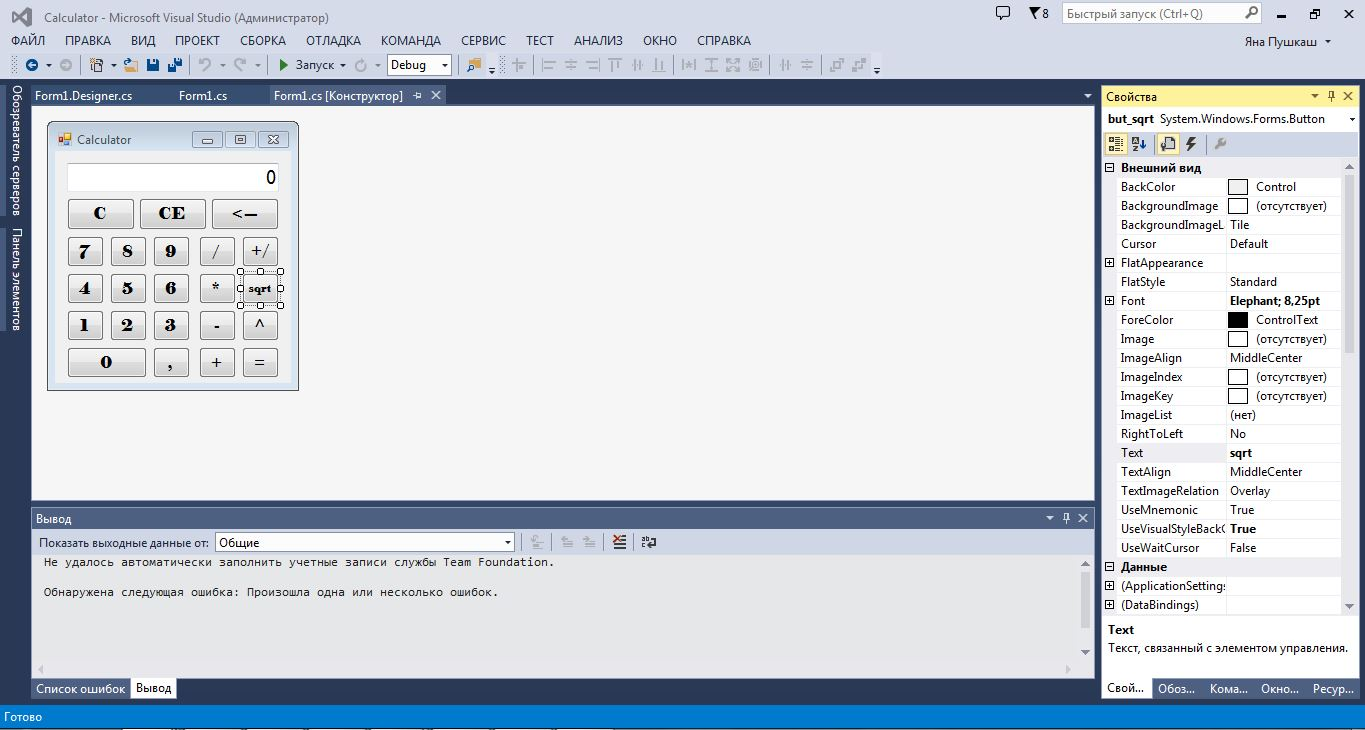
\includegraphics[width=1\linewidth]{images/Constructor.jpg}}
	\caption{Microsoft Visual Studio Constructor}
	\label{ris:image}
\end{figure}
\hfill
\begin{figure}[h]
	\center{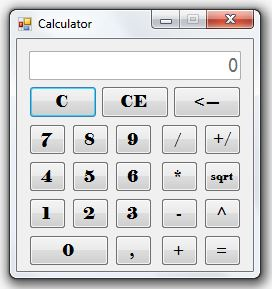
\includegraphics[width=0.5\linewidth]{images/Calculator.jpg}}
	\caption{Калькулятор}
	\label{ris:image}
\end{figure}

\clearpage